\subsection{Physical Structure}
The structure of the robot should allow the movement of the robot across the map. 
That means, the robot should have at least two motors to move in the plane of the circuit and a minimum of two light sensors to check its position referred to the black lines of the map and check when the robot has arrived to a crossroad.

\subsubsection{Motor configuration and control}
The chosen motor configuration uses two motors to drive two parallel wheels. 
This allows the robot to change the direction of the movement setting a different duty cycle on each motor.

To follow a line, the robot should be able to turn depending on how far from the center of the line it is.
The two motors should hence be set to different speeds while driving to account for the robot leaving the line.
These speeds are chosen with a P controller.
This controller slows down the speed of one or another wheel in relation to the displacement of the sensors from the line. 


\subsubsection{Sensor configuration}

Three light sensors are used. 
Two of them are used in the line following control and are placed in the front of the robot.
The distance between them is 40mm, which is bigger than the line width.
This gives to the controller a big actuation range, as the distance between the sensors is bigger than the width of the line.

In the position control, the value of the sensors are compared.
These values should then be equal when the robot is centred above the line
and both sensors should be low when the robot is facing a crossroad.

The third sensor is placed in the rear end of the robot, just before the wheels.
It is used to detect the lines of the crossroads when going back and turning.

This sensor is placed the closest possible to the wheels axis and far away from the robot center so it is not affected by the followed line.

Since the light sensors highly sensitive to changes in the ambient light levels, especially under sunlight exposure, a shielding from such is needed.
To solve this problem, first a shield around the three sensors is added such that the ambient light does not affect the measurements.
This gives good results in the laboratory and under sunlight on cloudy days, but is unable to work on sunny days as the sensors are still affected by the high intensity of the sun.
To minimize the effect of the sun, a second shield is placed covering the robots base, so the sensors are always in the shadow.
This system has shown good results under all conditions.
This shielding is shown on figure \ref{fig:robotImage}.



\subsubsection{Tool configuration}

To be able to push and guide the can across the map, the robot should have a proper tool that allows this task. 
The proposed design consist of two bars placed at an angle to each other such that the can is guided to the center when driving straight forward.
This configuration allows catching the can even when its displaced from the crossings, making the robots job simpler.

Considering the rules of the game then the can is not permitted to be pushed left or right and because of that, no special design enabling this is required.


The final build of the robot is seen in figure \ref{fig:robotImage}.

\begin{figure}[H]
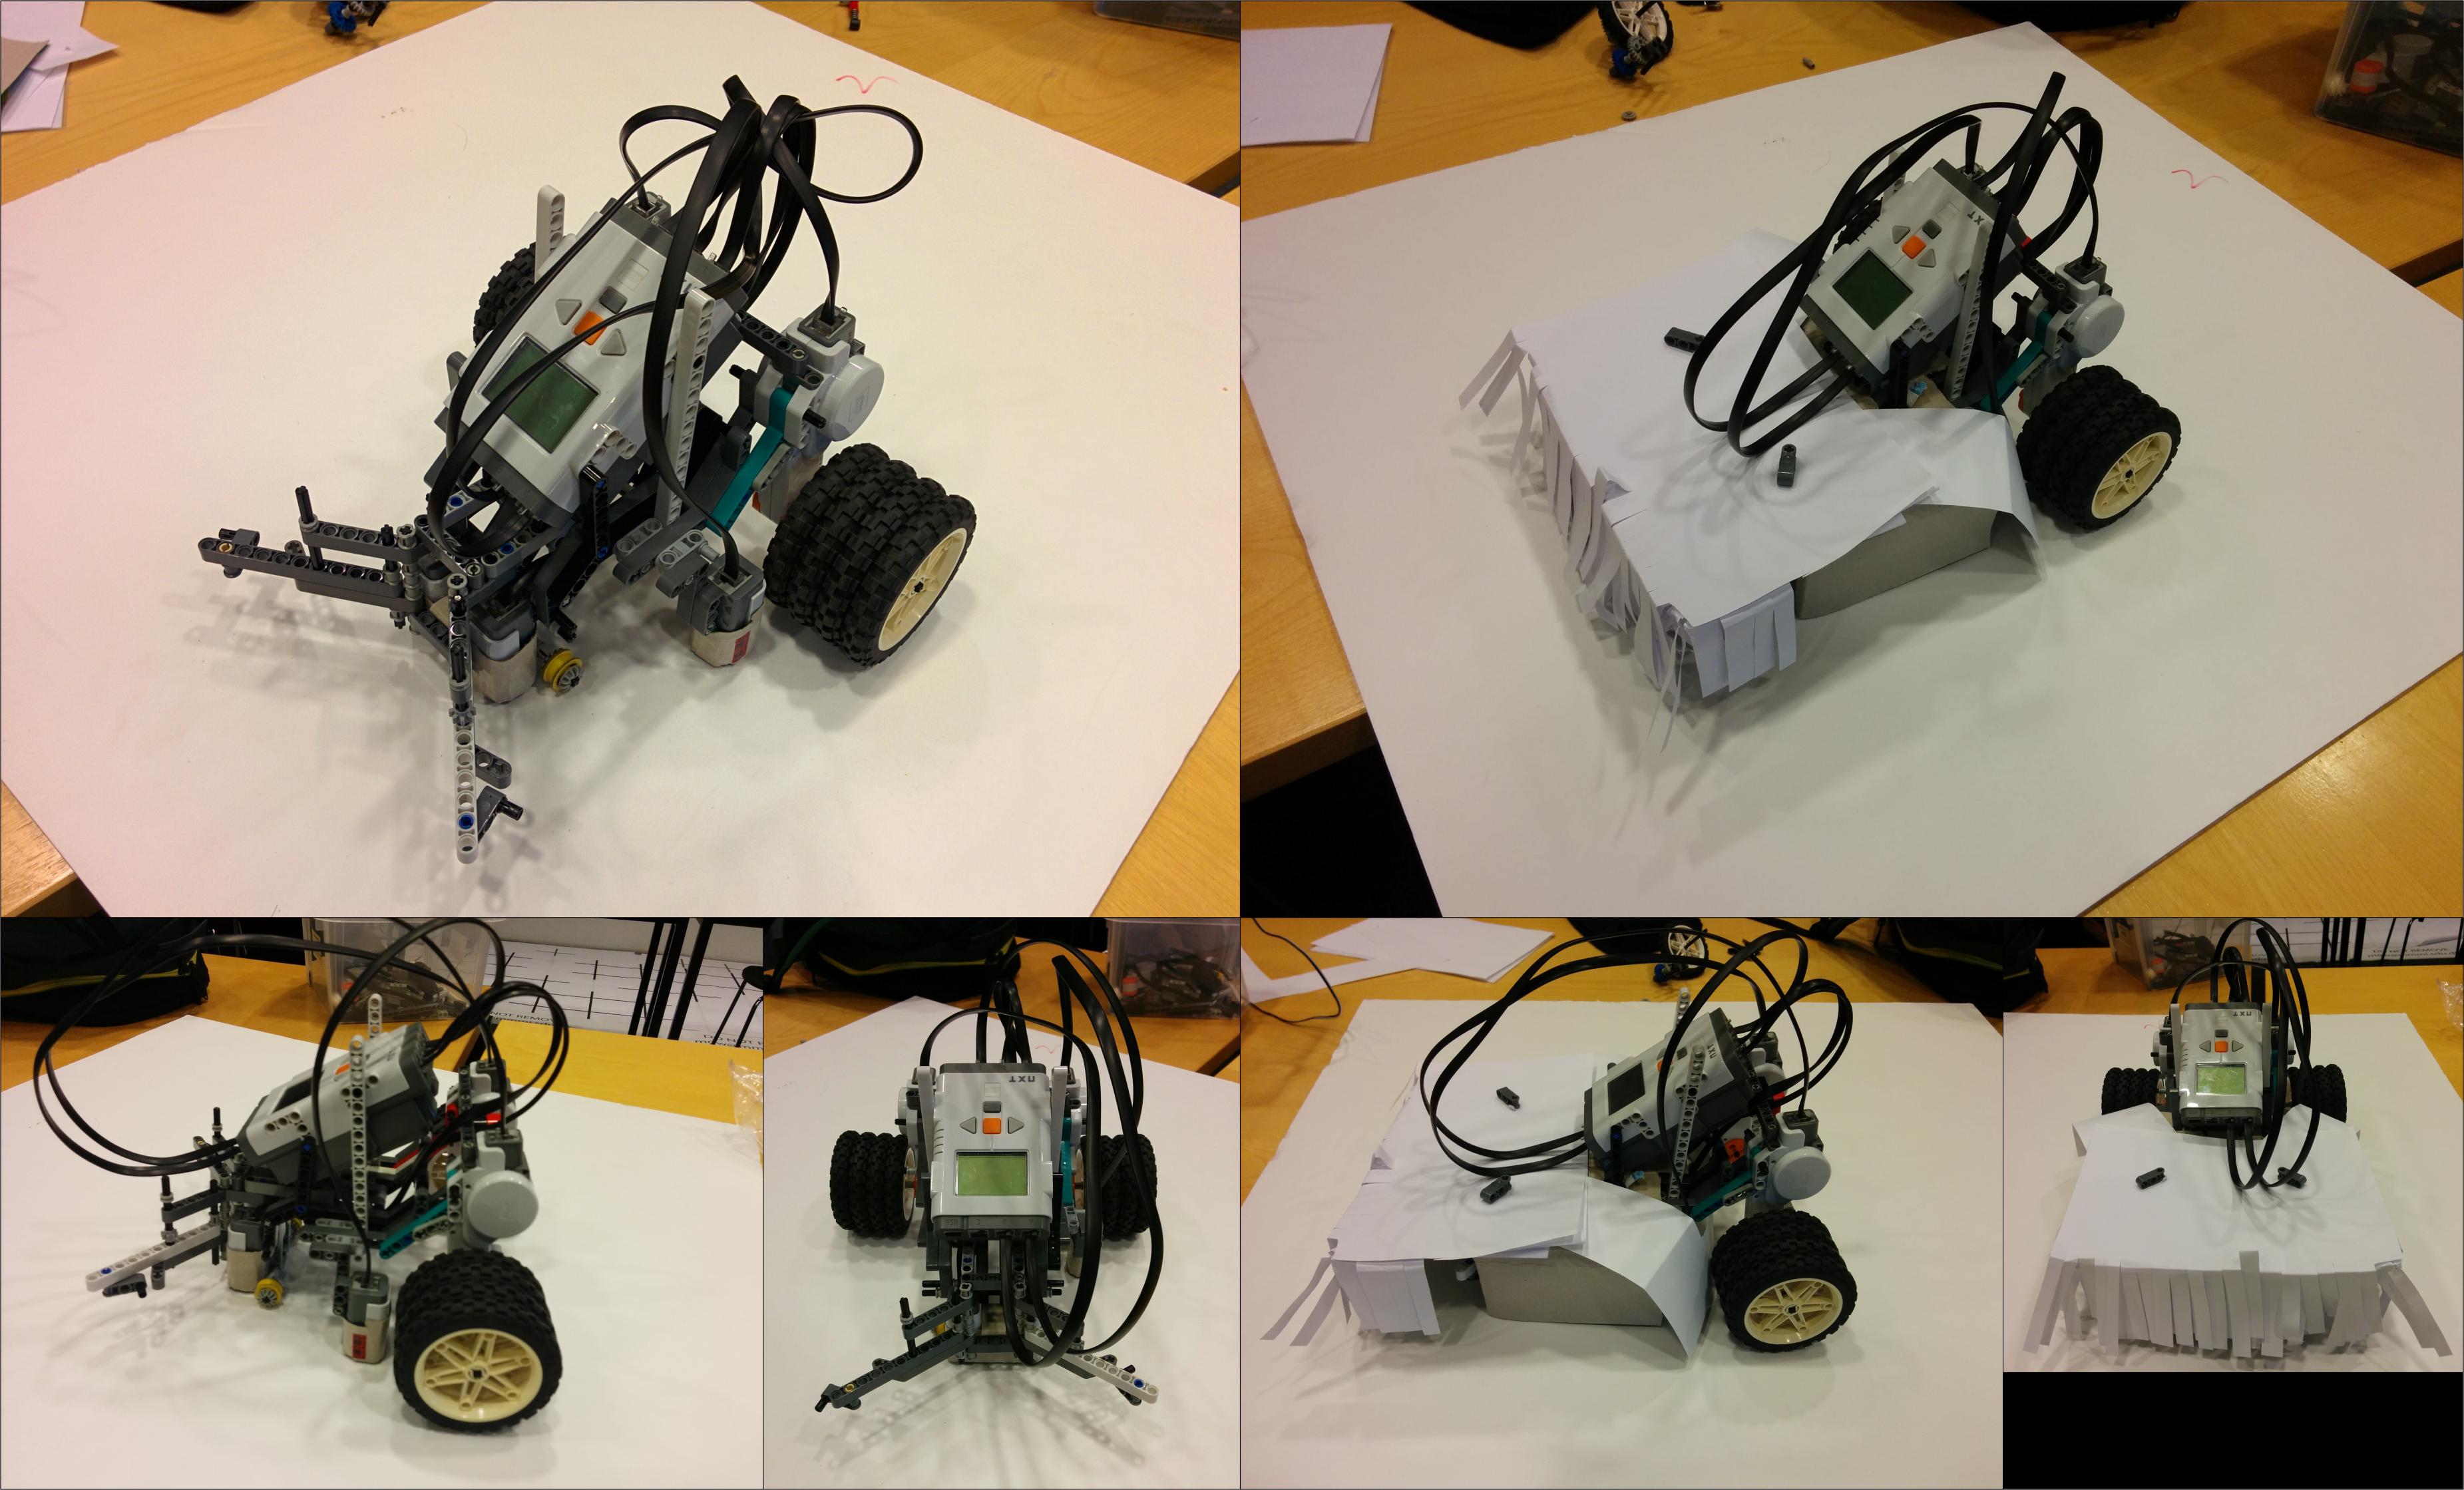
\includegraphics[width=10cm]{sokobanRobotImage.png}
\centering
\caption[Images of the built robot.]{Images of the built robot. Left, the robot without shielding. Right, the shielded robot.}
\label{fig:robotImage}
\end{figure}

